\section{Fretboard}

\begin{minipage}{0.48\textwidth}
Each position on the neck has a different pitch. The metal bars on the neck are called the \textbf{frets}.

For example, if someone asks to press the 2nd fret on the 3rd string, then you press you finger in the area of the green dot. Right next to the fret. See \ref{fig:guitar_string_fretting}.
\end{minipage}
\hfill
\begin{minipage}{0.48\textwidth}
    \centering
    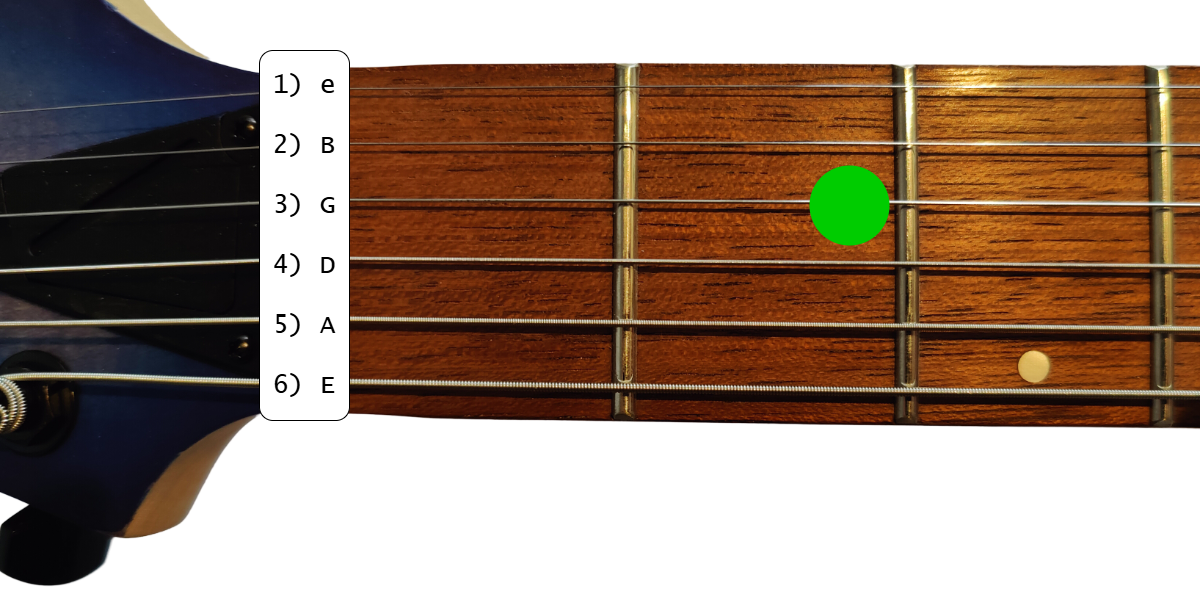
\includegraphics[width=\textwidth]{../../Images/guitar-neck-fretting.png}
    \captionof{figure}{The green dot in the finger placement for the 2nd fret on the 3rd string}
    \label{fig:guitar_string_fretting}
\end{minipage}

In music there are 12 different pitches before coming 'back around'. When you come back at the same note letter you are an octave higher. The 12 different notes are shown below.

\begin{table}[h]
\centering
\begin{tabular}{*{12}{P{5mm}}}
\large{A} & \large{A\sharp} & \large{B} & \large{C} & \large{C\sharp} & \large{D} & \large{D\sharp} & \large{E} & \large{F} & \large{F\sharp} & \large{G} & \large{G\sharp}
\end{tabular}
\end{table}

You may see that there are only \textbf{7} different letters and \textbf{5} letters with a \textbf{\sharp}. These \sharp symbols are called \textbf{sharps}. On the fretboard a \sharp means you move one fret up (to the body of the guitar).

\infobox{The reason that there are not just 12 different letters like "A, B, C, D, E, F, G, H, I, J, K, L", has to do with the history of music.}

In \ref{fig:guitar_string_a_octave} you see a music staff with underneath it tablature (TAB). In the next section we will learn to read the notes. For now you can try to read the tabs first to play the sequence.

Each line in the TAB section represents a guitar string, with the 6th (thickest) string on the bottom. The numbers indicate which fret should be pressed (a 0 means an open string). So the TAB in \ref{fig:guitar_string_a_octave} says to first play an open A string, and then play each ascending fret up to the 12th fret.

\begin{figure}[h]
    \centering
    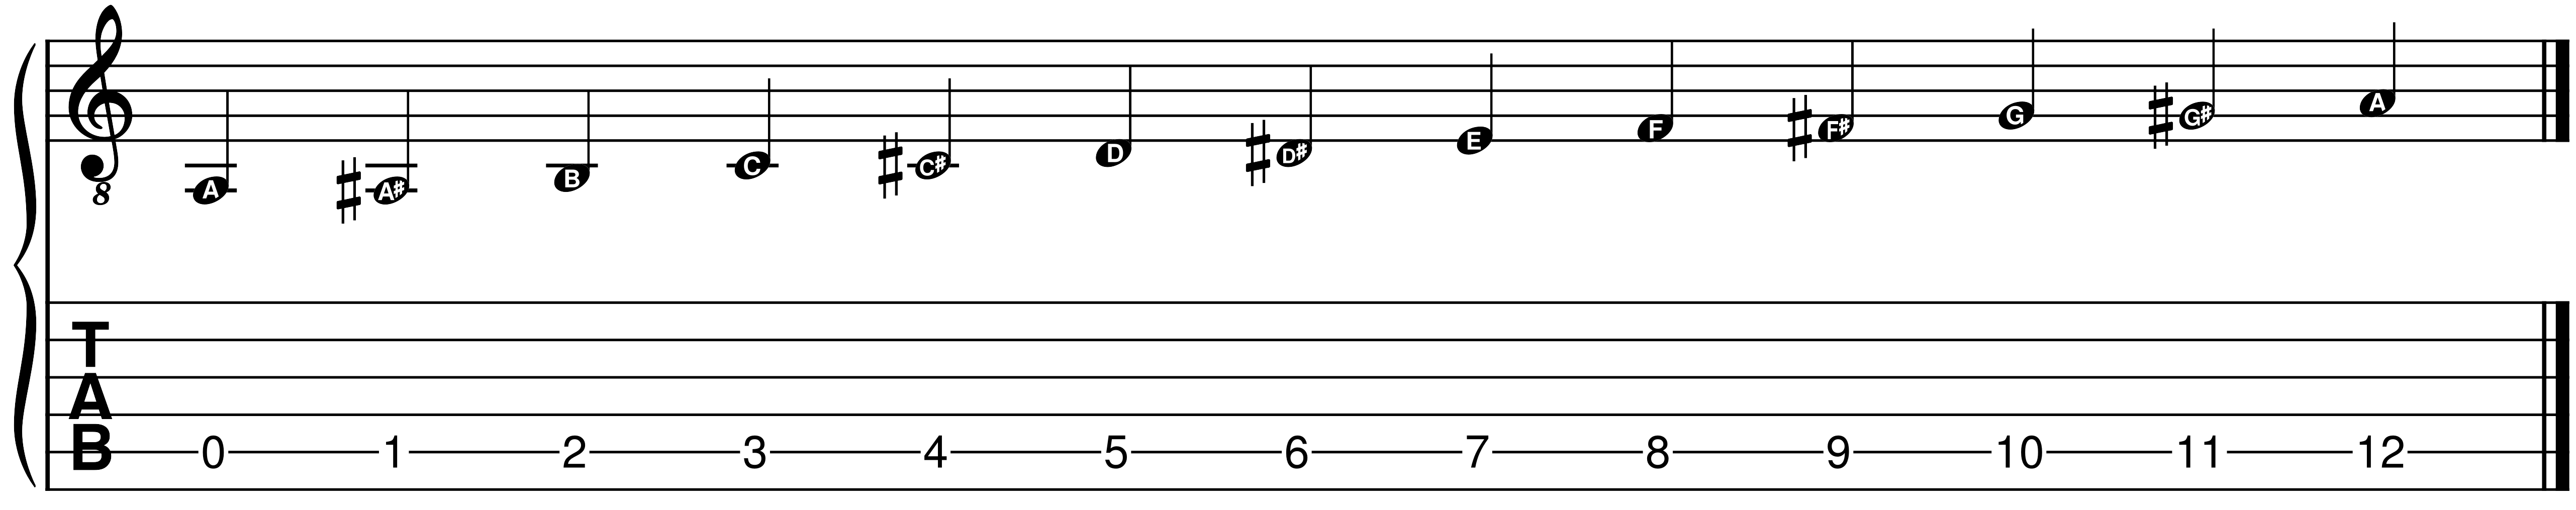
\includegraphics[width=\textwidth]{../../MuseScore/Guitar/PitchesSharps.png}
    \caption{An octave from A to A on the 5th A string}
    \label{fig:guitar_string_a_octave}
\end{figure}

% TODO: octave of multiple string and flats/naturals